\documentclass[../main.tex]{subfiles}

\begin{document}

\section{Random Matrix Theory}
A lot of physical systems -- e.g. systems with glassy dynamics -- can often be modeled using graphs.
This makes graph theory an integral part of physics itself and it has been studied extensively.
In this exercise we will look at such systems that additionally contain disorder. 
Every regular graph can be expressed as an adjacency matrix which can be used to analyze the system.
\par

\subsection{Analysis by Direct Diagonalization}

\subsubsection{Sparse Random Matrix}
In the first step of our analysis we use well known techniques to establish a baseline for our methodology.
The method we use is called Direct Diagonalization and it obtains the spectrum of the system by using numeric Exact Diagonalization (ED).
\par 

\begin{figure}[htpb]
    \centering
    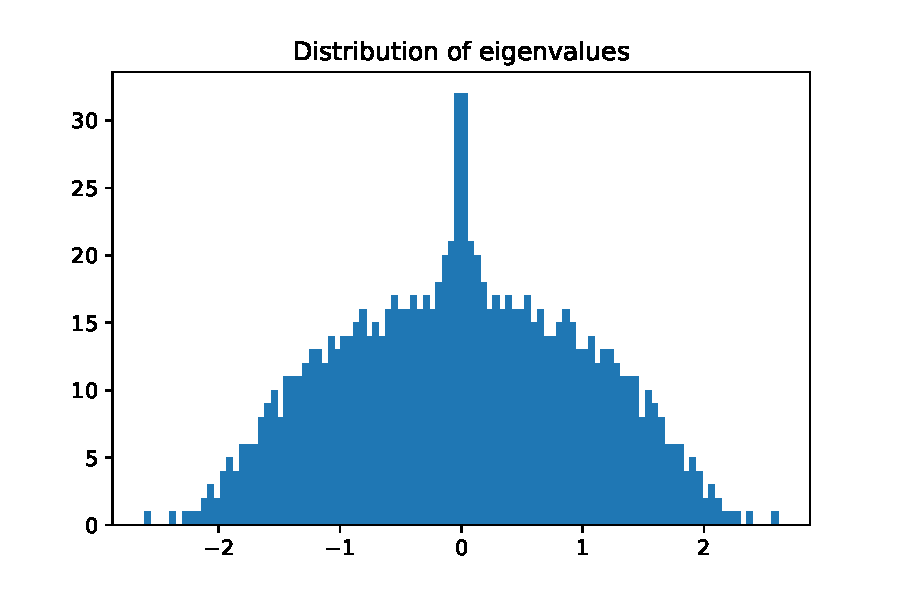
\includegraphics[width=0.8\textwidth]{../figures/2_1_1_spectrum_sparse.pdf}
    \caption{Spectrum of a RRG of size $2^{10}$ with connectivity 3 averaged over 10 different realizations.}
    \label{fig:spectrum_sparse}
\end{figure}

In a first analysis step we generate 10 different Random Regular Graphs (RRG) and calculate their spectrum vie ED and average their spectrum.
In Figure \ref{fig:spectrum_sparse} you can see the spectrum of the RRG's adjacency matrices of size $N = 2^{10}$ with connectivity 3 averaged over 10 different realizations.


\subsubsection{Fully Connected Graph}

Next we want to analyze the spectrum of a fully connected network. For this we gain generate an adjacency matrix multiply it's components with gaussian noise scaled by $c = N-1$.

\begin{figure}[htpb]
    \centering
    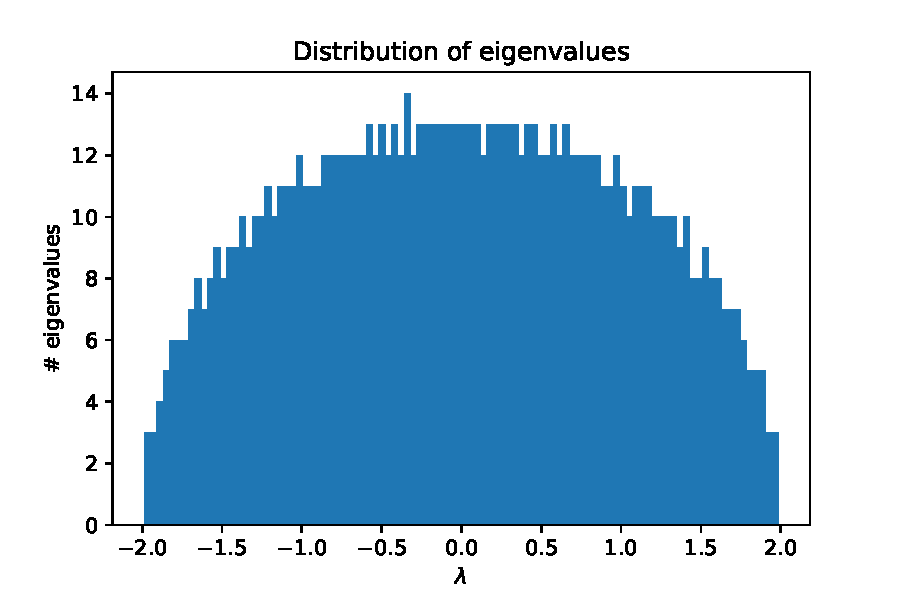
\includegraphics[width=0.8\textwidth]{../figures/2_1_2_spectrum_full.pdf}
    \caption{Spectrum of a fully connected network of size $N = 2^{10}$ ($c = N-1$) averaged over 10 different realizations.}
    \label{fig:spectrum_full}
\end{figure}

In Figure \ref{fig:spectrum_full} we can see the spectrum of the fully connected network averaged over 10 realizations of the Random Graph.



\subsubsection{Large Matrix limit}

As the number of nodes in the fully connected graph increases we expect the self-averaging effects of the system to become stronger.
This means that the density of our spectrum will more closely the exact solution in the $N\to \infty$ limit.
That solution is given by the Wigner-Semicircle law, which states that the density of eigenvalues describes a semicircle described by 

\begin{align}\label{eq:wigner_semicircle}
    \rho(\lambda) = \frac{\sqrt{4 - \lambda^2} }{2 \pi}
.\end{align}


\begin{figure}[htpb]
    \centering
    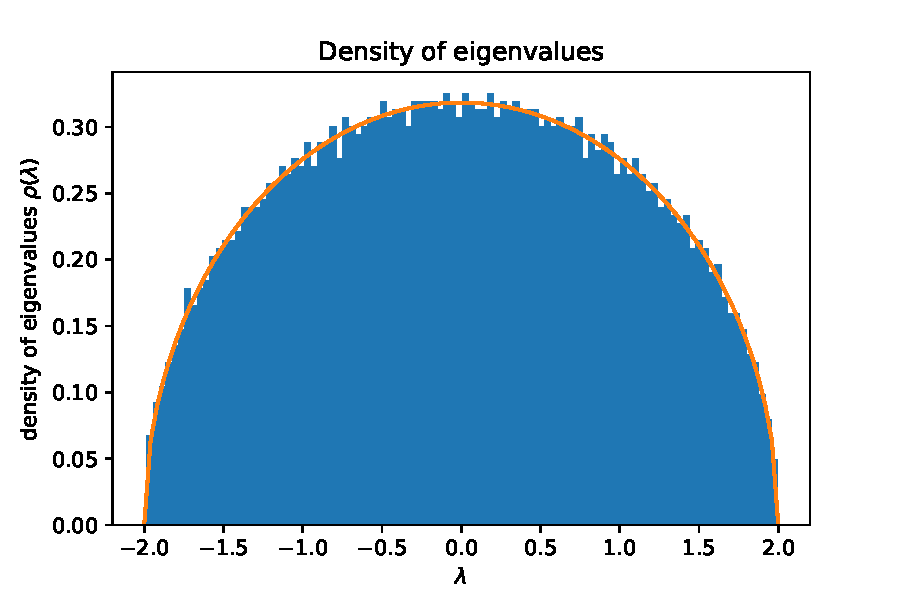
\includegraphics[width=0.8\textwidth]{../figures/2_1_3_wigner_semicircle.pdf}
    \caption{
        \emph{Spectral density} of a fully connected network of size $N= 2^{12}$ of a single realization of a single realization.
        Furthermore we overlayed the semicircle defined given by the Wigner-Semicircle law from eq. \eqref{eq:wigner_semicircle}.
    }
    \label{fig:wigner_semicircle}
\end{figure}

\subsubsection{Universality Classes}
As graphs with a high connectivity $c$ have very similar topology and their behavior is self-averaging, we can classify them by their spectral properties.

\begin{figure*}[htpb]
    \thisfloatpagestyle{empty}
    \vspace{-3cm}
    \centering
    \begin{subfigure}{\textwidth}
        \centering
        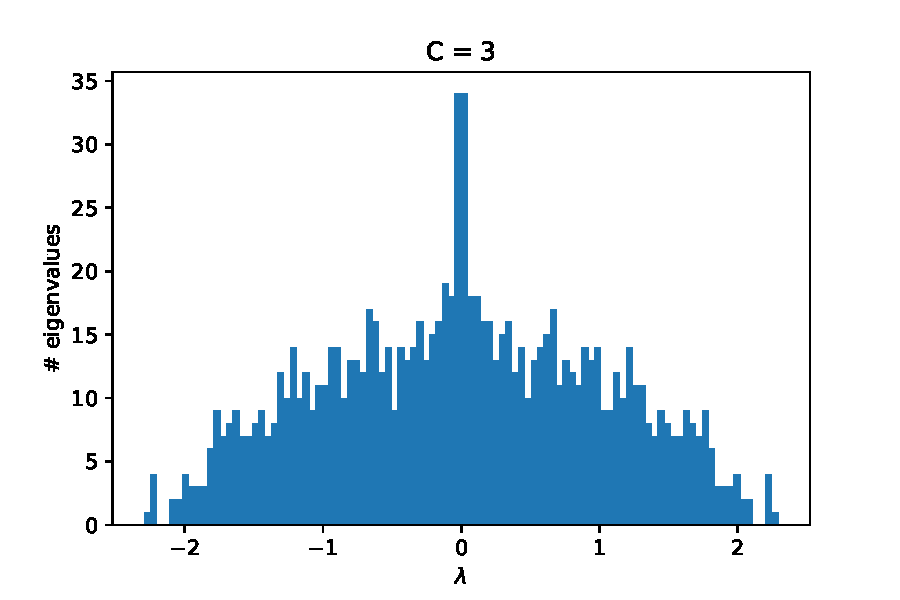
\includegraphics[width=.8\linewidth]{../figures/2_1_4_universality_classes0003.pdf}
        \caption{}
        \label{fig:universality_classes_0003}
    \end{subfigure}\\%
    \begin{subfigure}{\textwidth}
        \centering
        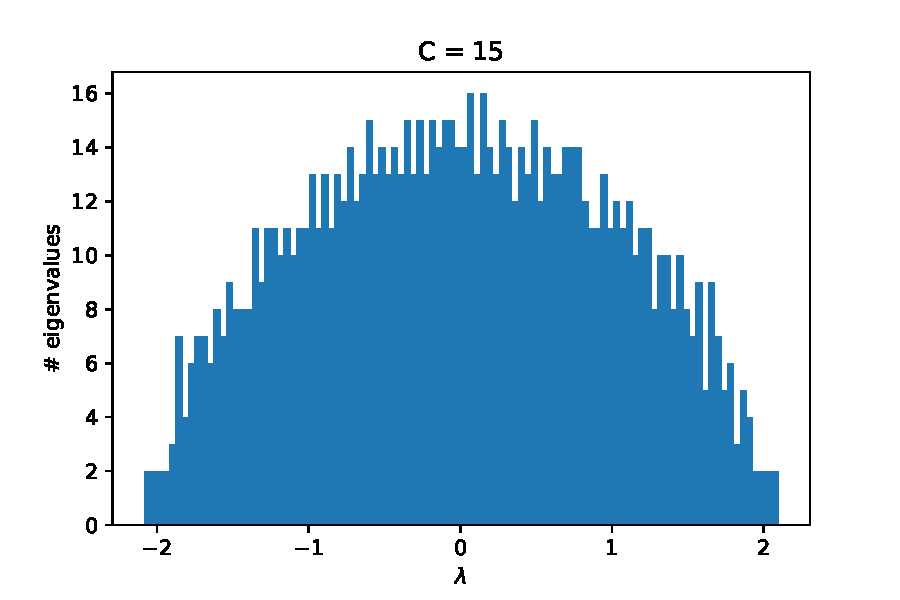
\includegraphics[width=.8\linewidth]{../figures/2_1_4_universality_classes0015.pdf}
        \caption{}
        \label{fig:universality_classes_0015}
    \end{subfigure}\\%
    \begin{subfigure}{\textwidth}
        \centering
        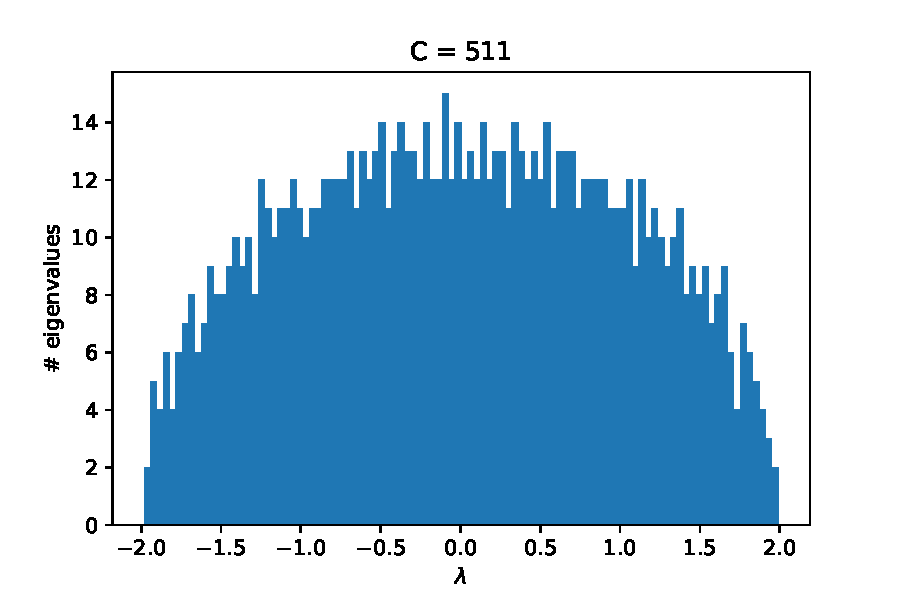
\includegraphics[width=.8\linewidth]{../figures/2_1_4_universality_classes0511.pdf}
        \caption{}
        \label{fig:universality_classes_0511}
    \end{subfigure}
    \caption{Spectrum of RRGs of size $N=2^{10}$ with different connectivities $c$.}
    \label{fig:universality_classes}
\end{figure*}

In Figures \ref{fig:universality_classes_0003}-\ref{fig:universality_classes_0511} we can see that already for quite small connectivities we get spectra that look very close to a semi-circle.
We can see that our idea that high connectivities should belong to the same class of spectrum does clearly hold.


\subsection{Analysis by Cavity Method}
\setcounter{subsubsection}{4}

\subsubsection{Update equation for the cavity precisions}

To calculate the cavity precisions of the Random Matrix problem we again impose gaussian distributions for our cavity and marginal probabilities.
This allows us to obtain recursive relations for the cavity and marginal precisions (inverse variances).

We can easily do so by inserting our assumptions into equations (18) and (19) on the exercise sheet.
The resulting equation for the cavity precision $\omega^{(j)}_k$ at some site $k$, given some cavity at site $j$ is 
\begin{align}
\label{eq:cavity_precs}
    \omega^{(j)}_k = i(\lambda - i \epsilon) + 
    \sum\limits_{l \in \partial k \setminus j }^{ } M^2_{ kl }/ \omega^{(k)}_l 
.\end{align}
$M_{ kl } $ is the value of the given random adjacency matrix representing the edge between site $k$ and $l$.

In similar fashion we can also obtain an equation for the marginal precisions $\omega_k$ at site $k$
\begin{align}
\label{eq:marginals_precs}
    \omega_k = i(\lambda - i \epsilon) + 
    \sum\limits_{l \in \partial k}^{ } M^2_{ kl }/ \omega_l 
.\end{align}

\subsubsection{Cavity method for sparse matrices}

\subsubsection{Mean-Field limit}

In the mean-field limit for the fully connected graph we assume $N \to \infty$.
We can see from equation \eqref{eq:cavity_precs} that -- in this limit and on a fully connected graph -- the single term left out scales as $\mathcal{O}(1)$, while the entire sum scales as $\mathcal{O}(N)$.
As $N$ grows, we will find that it will be increasingly less significant whether we will be looking at the marginals or the cavity distributions.

\subsubsection{Mean Resolvent}



\ifSubfilesClassLoaded{
	% if it's compiled alone
}{
	% if it's compiled in the main file
    \newpage
}
\end{document}
